\chapter{Einleitung}
\label{cha:Einleitung}

\section{Motivation}

Die vorliegende Masterarbeit ist Teil des Forschungsfeldes der Arbeitsgruppe Brendel\footnote{\url{https://www.uni-marburg.de/fb20/haematoonkol/forschung/brendel}}, des \emph{Universitätsklinikums Gießen und Marburg}, welche sich mit \ac{AML} befasst, in Kooperation mit der \emph{Bioinformatics and Systems Biology Group} der Justus-Liebig-Universität Gießen\footnote{\url{https://www.uni-giessen.de/fbz/fb08/Inst/bioinformatik}}. Ziel dieser Arbeit ist es, zu testen ob die Theorie der \ac{APs} zur Annotation von \ac{SNPs}, in spezifischen Regionen, im Genom von \ac{AML} Patienten angewendet werden kann.

Bei den \ac{APs} handelt es sich um eine Methode der Transformation der physikochemischen und wechselwirkenden Eigenschaften der Proteinstruktur in ein Energiemaß. So können 3D Strukturinformationen in eindimensionale Energiewerte überführt werden, mit denen leichter gerechnet werden kann. Diese jeweiligen Energiewerte der Proteine liegen in sogenannten \ac{EPs} vor und können als Grundlage für proteomische Untersuchungen dienen. Die Theorie hinter den Aminosäurerest-Pseudopotentialen existiert schon länger, jedoch wurde sie bisher nicht zur Annotation von potentiell pathogenen \ac{SNPs} eingesetzt. Die Theorie ermöglicht es uns mehr Informationen aus der Proteinstruktur verwenden zu können, da im biologischen Kontext die korrekte Faltung der Proteine eine sehr wichtige Rolle spielt. Ein Austausch einer Aminosäure könnte somit die Faltung verändern und das Protein beschädigen. 

Bisher ist die Abfolge der Aminosäuresequenz die größte Informationsquelle etablierter proteomischer Analyseverfahren \cite{Landels.2015}. Diese jedoch spiegelt nur einen Teil der gesamten biologischen Information der Polypeptidkette wieder. Um ein tiefer gehendes Verständnis für das biologische System zu entwickeln ist es notwendig alle möglichen Informationen einfließen zu lassen, auch die 3D Struktur. Die Verwendung der 3D Struktur führt jedoch zu einem drastisch erhöhten Aufwand, weswegen es bisher in den meisten Fällen nicht praktikabel war. Durch die Aminosäurerest-Pseudopotentiale lässt sich dieser Mehraufwand erheblich reduzieren, indem die bisherige Aminosäuresequenz durch \ac{EPs} erweitert wird. Diese Energieprofile stellen ein eindimensionales Maß dar, welches den Rechenaufwand erheblich reduziert. Zudem sind sie leichter zu lesen und zu interpretieren, sodass die 3D Strukturinformationen für die Analysen nutzbar sind.

In einer vorherigen Arbeit mit dem Titel \emph{Entwicklung mole\-kular-phylo\-genetisch\-er Methoden auf Grundlage von Aminosäurerest- Pseudopotentialen}, wurde gezeigt, dass es möglich ist die Information, der 3D Strukturen, aus der \ac{PDB} und \ac{Pfam} zu nutzen\cite{Mathias.2014}. Um aus der Proteinstruktur, mit den Informationen aus den EPs eine Substitutionsmatrix zu kalkulieren, welche die zusätzlichen Informationen der \ac{APs} nutzbar macht. Es wurde durch den Vergleich mit anderen Substitutionsmatritzen gezeigt, dass \ac{EPs} mindestens äquivalent zu den etablierten Ansätzen, wenn nicht sogar besser sind. Als Fazit dieser Arbeit wurde festgehalten, dass sich \ac{EPs} als Datengrundlage eignen, um den Informationsgehalt von einfachen Sequenzen zu erweitern.


\section{Leukämie}
Leukämie ist entweder eine maligne Erkrankung des Knochenmarks bzw. des blutbildenden Systems oder des lymphatischen Systems. Es wird aktuell in vier Unterarten der Leukämie unterschieden, der Plasmazellenleukämie, der lymphatischen Leukämie, der Monozytenleukämie und der myeloischen Leukämie. Zudem gibt es eine Unterteilung in \emph{chronisch}, meist mehrere Jahre andauernde Erkrankung und \emph{akut}, welche eine schnelle und aggressive Form der Erkrankung darstellt.

Die Leukämie wird nach der Art der beteiligten Zellen klassifiziert. Patienten mit \ac{AML} haben eine Störung der Myelopoese, welches für die Bildung von Granulozyten, Monozyten, Erythrozyten und Megakaryozyten zuständig ist. Lymphatische Leukämien betreffen hingegen die Lymphozyten und deren Vorläuferzellen. Die Blutstammzellen verlieren bei \ac{AML} die Fähigkeit sich in Blutzellen auszudifferenzieren, zudem proliferieren sie unkontrolliert im Knochenmark\cite{Papaemmanuil.2016}. Schließlich treten undifferenzierte \emph{Blasten} (auch Leukämiezellen genannt) aus dem Knochenmark ins periphere Blut über und verdrängen dort die gesunden Zellen. Durch diese Verdrängung der normalen Blutbestandsteile entsteht ein Mangel an Sauerstoff, eine sogenannte Anämie. Weitere Symptome können ein Gefühl der Erschöpfung, Blutarmut, Hämatome und eine Schwächung des Immunsystems sein. Die \ac{AML} ist eine lebensbedrohliche Krankheit und ist unbehandelt innerhalb weniger Wochen letal. Zusätzlich können Blasten noch andere Organe wie Leber, Milz und Lymphknoten befallen und so deren Funktionen stören.

Die Diagnostik einer Leukämie wird durch die Klassifikation der Blasten ermöglicht, indem die morphologischen Eigenschaften der Blasten untersucht werden. Dafür wird dem Patienten eine Blutprobe entnommen und unter dem Mikroskop analysiert. Ausschlaggebend für eine Diagnostik ist unter anderem der Grad der Differenzierung, denn bei chronischen Leukämien lassen sich vermehrt Blutzellen beobachten, welche fast komplett ausdifferenziert sind, wohingegen bei einer akuten Leukämie vor allem undifferenzierte Blutzellen zu beobachten sind\footnote{\url{https://www.cancer.org/cancer/acute-lymphocytic-leukemia/about/what-is-all.html}}. Um eine endgültige Diagnose zu stellen ist aber immer eine Knochenmarkspunktion nötig. Neben den morphologischen Eigenschaften werden die Zellen zusätzlich molekularbiologisch untersucht, indem zur Risikoeinstufung der Karyotyp bestimmt wird. In der AG Brendel wird zusätzlich noch eine Mutationsanalyse von ausgewählten Genen wie z.B. FLT3, IDH1, KRAS \& NRAS des Illumina TruSight Myeloid Sequencing Panel vollzogen.

\begin{figure}
\centering
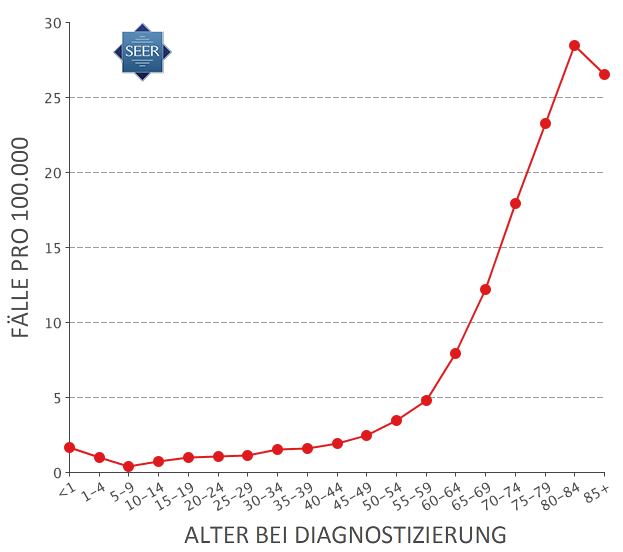
\includegraphics[width=.95\textwidth]{images/Alter_AML_2014.png}
\caption{Zu sehen ist die Wahrscheinlichkeit des Auftretens einer \ac{AML} in Abhängigkeit vom Alter, übergreifend über alle Abstammungen und Geschlechter. Daten aus dem SEER\cite{Howlader.2014} Explorer\protect\footnotemark{} von 2010 bis 2014.}
\label{fig:Alter_AML}
\end{figure}
\footnotetext{\url{https://seer.cancer.gov/explorer/}}
Eine Leukämie kann in jeder Altersstufe auftreten, doch es gibt spezifische Altersgruppen in denen spezielle Arten der Leukämie wahrscheinlicher sind, siehe \ref{fig:Age_AML_ALL}. So treten im Kindesalter hauptsächlich \ac{ALL} auf\cite{Rubnitz.2012}, im Erwachsenenalter hingegen ist eine \ac{AML} die wahrscheinlichste Erkrankung, siehe \ref{fig:Alter_AML}. Generell lässt sich sagen, dass die Wahrscheinlichkeit an einer Leukämie zu erkranken, sich mit dem Alter erhöht, geschuldet durch Mutationen die sich im Laufe des Lebens in den Zellen akkumulieren.

\begin{figure}
\centering
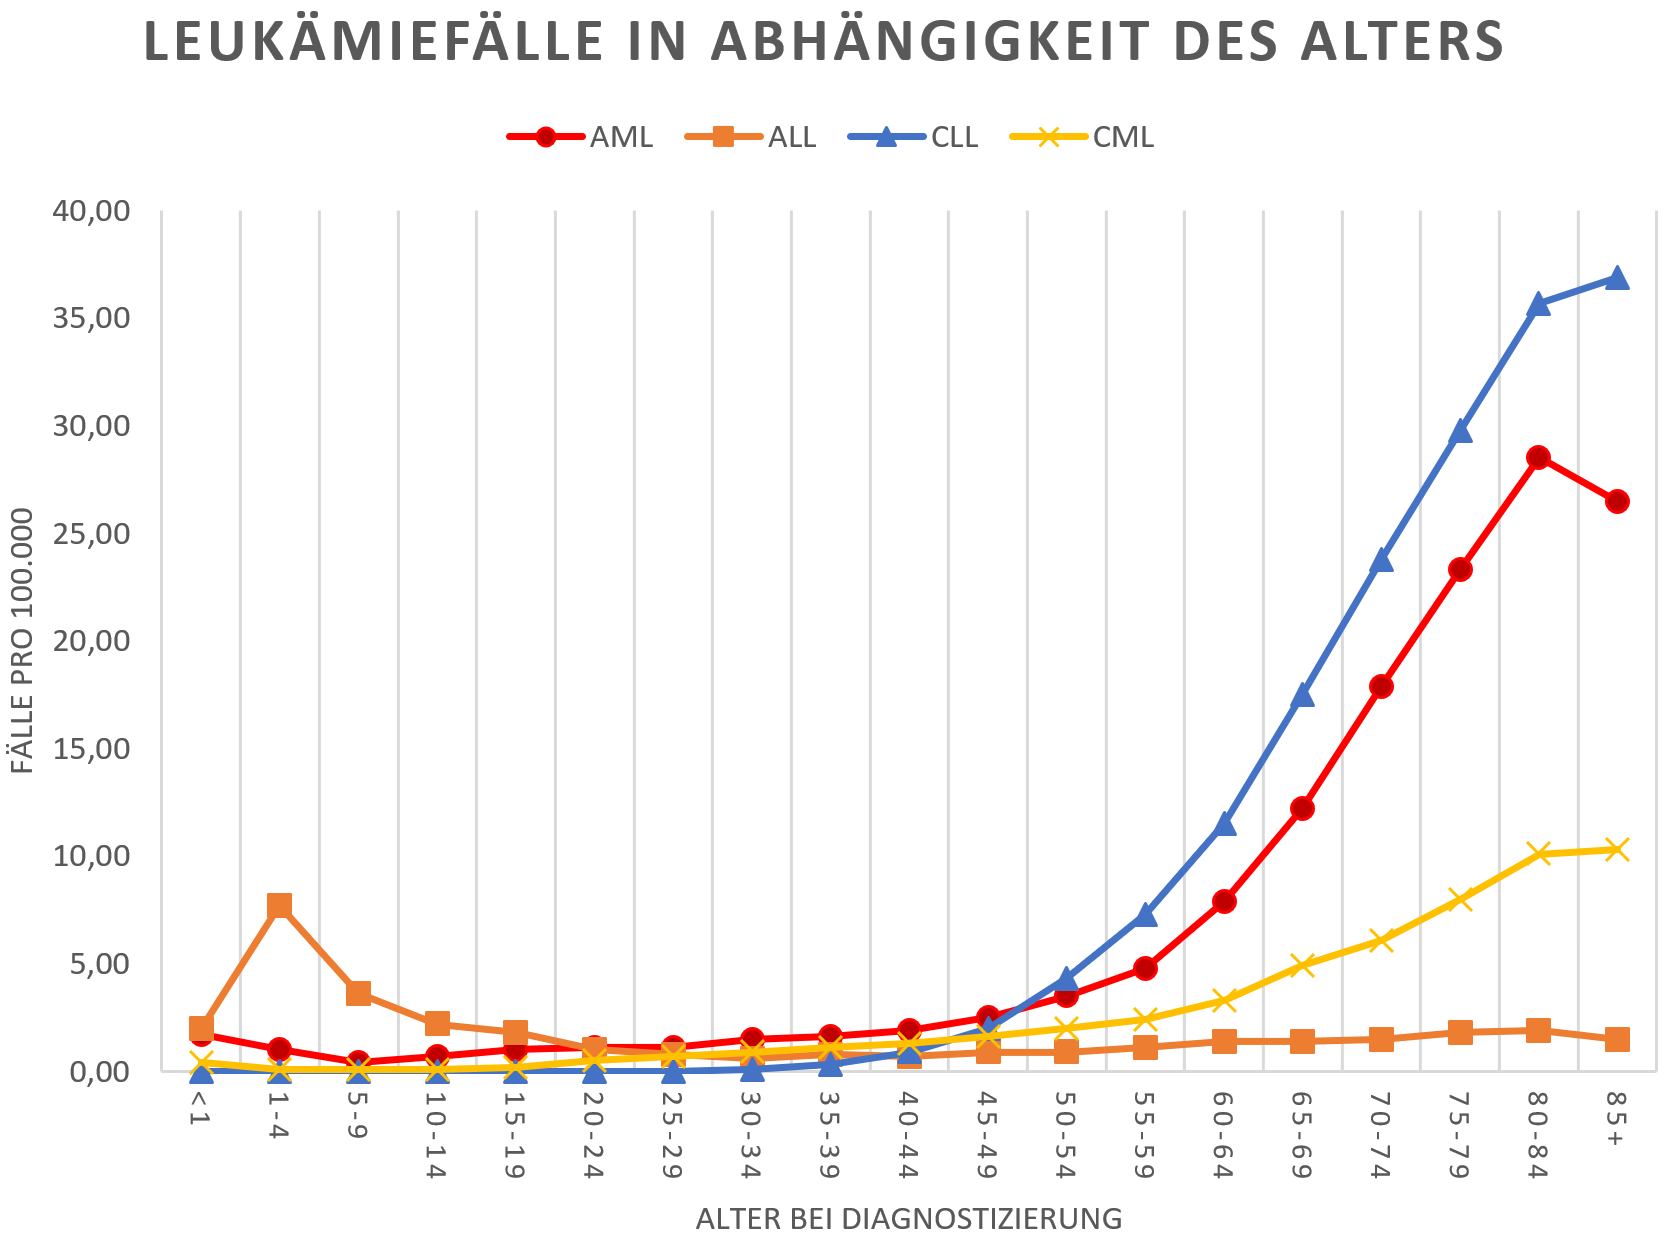
\includegraphics[width=.95\textwidth]{images/leukaemie_faelle_nach_alter.png}
\caption{Dargestellt ist die Wahrscheinlichkeit des Auftretens einer speziellen Leukämie in Abhängigkeit zum Alter unabhängig vom Geschlecht oder der Abstammung. Daten aus dem SEER 2010-2014.}
\label{fig:Age_AML_ALL}
\end{figure}

Leukämie entsteht durch genetische Veränderungen in undifferenzierten Blutstammzellen. Wenn die Mutationen in speziellen Regionen liegen\cite{Wakita.2016}, so teilen sich die Zellen unkontrolliert und sind in ihrer Funktion stark eingeschränkt. Es genügt bereits eine kleine Veränderung in einer der Stammzellen, damit deren Tochterzellen die gesunden Zellen verdrängen. Die Ursachen für diese genetische Modifikation sind im großen noch unbekannt, im allgemeinen wird jedoch vermutet, dass die spezifischen Risikofaktoren welche Krebs begünstigen auch eine Leukämie verursachen können\cite{Petit.2014}. Durch die technische Weiterentwicklung der Länder und der damit verbundenen erhöhten Population und Lebensspanne der Menschen, steigt die Anzahl der Krebserkrankungen. Hierbei spielen Alter, Rauchen, Übergewicht, sportliche Aktivität und Reproduktionsverhalten geprägt durch die Urbanisierung eine zentrale Rolle\cite{Torre.2015}. Des Weiteren ist die Aussetzung spezieller Strahlung, z.B. ionisierende Strahlung oder passive Radon Strahlung, sowie mutagene Chemikalien, diverse Viren und genetische Vorbelastung im Verdacht krebserregend zu sein.

Therapiert wird \ac{AML} mit Zytostatika und einer allogenen Knochenmark- bzw. Stammzelltransplantation\cite{Cheson.2003}. Bei der Stamm\-zell\-trans\-plan\-tat\-ion wird das erkrankte Knochenmark durch gesunde Zellen von einem passenden Spender ersetzt. Die Stammzellen werden dem Spender, nach einer Medikation, aus dem Blut extrahiert und dem Empfänger, nach einer Chemotherapie oder Bestrahlung, mittels Transfusion übertragen. 

Nach Therapiebeginn sind die Leukämiezellen nicht mehr unter dem Mikroskop nachweisbar. Die Molekulargenetik bietet daher die Möglichkeit den Erkrankungsverlauf durch die Bestimmung der so genannten minimalen Resterkrankung \ac{MRD} zu verfolgen. Durch die \ac{MRD} lassen sich Leukämiezellen schon ab 0,01\% im Blut nachweisen.

Nach einer Therapie gehen die meisten Menschen in Remission, dies bedeutet, dass die Symptome der \ac{AML} zurück gehen und sie aus dem Krankenhaus entlassen werden können. Doch leider hat \ac{AML} eine hohe Rückfallquote, welche stark abhängig vom Alter ist. So dass im Schnitt 5 Jahre nach der \ac{AML} Diagnose nur noch 26,9\% am Leben sind.

\begin{figure}
    \centering
    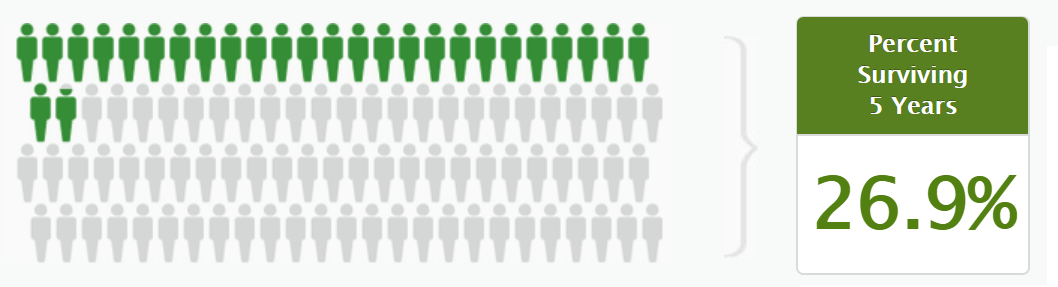
\includegraphics[width=.95\textwidth]{images/SEER_survival_rate_AML.png}
    \caption{Basierend auf Daten aus SEER 2007-2013. Graue Personen repräsentieren diejenigen, welche an \ac{AML} gestorben sind. Grüne repräsentieren diejenigen, die 5 Jahre oder mehr überlebt haben\protect\footnotemark{}.}
    \label{fig:seer_aml_rate}
\end{figure}
\footnotetext{Daten aus dem SEER \url{https://seer.cancer.gov/statfacts/html/leuks.html}}

Abbildung \ref{fig:seer_aml_rate} zeigt die relativen Überlebensraten von \ac{AML} Patienten. Diese vergleicht das Überleben von Patienten, welche mit Krebs diagnostiziert wurden, mit dem Überleben von Menschen in der allgemeinen Bevölkerung, die das gleiche Alter, Geschlecht und Abstammung aufweisen. 
%Da Überlebensraten auf großen Gruppen von Menschen basieren, können sie nicht dazu verwendet werden, genau vorherzusagen, was mit einem einzelnen Patienten passiert. Kein Patient gleicht dem anderen, und die Behandlung und das Ansprechen auf die Behandlung können sehr unterschiedlich sein.


%Das Ziel ist jede Mutation zuverlässig klassifizieren zu können.
%AML ist die Häufigste Erkrankung im Erwachsenen Alter
\section{Zielsetzung}

Im Universitätsklinikum Marburg in der AG Brendel wird mit dem \emph{Illumina TruSight Myeloid Sequencing Panel}\footnote{\url{https://www.illumina.com/products/by-type/clinical-research-products/trusight-myeloid.html}} gearbeitet, um \ac{AML} spezifische Regionen auf Mutationen zu untersuchen. Dieses Panel liefert nach dem Screening eine Tabelle mit allen Mutationen des Patienten und deren Lokalisation. Auffällig dabei ist, dass die meisten Mutationen in Form von \ac{SNPs} auftreten. Obwohl alle Patienten die gleichen Symptome einer \ac{AML} zeigen, sind die Meisten der detektierten \ac{SNPs} Patienten spezifisch und somit noch unbekannt und ihre Wirkung auf das entsprechende Gen kann nicht ermittelt werden. Dies hat zur Folge, dass keine Aussage über eine eventuelle Pathogenität und weiter deren Einfluss auf den Organismus getroffen werden kann. 

Ziel dieser Masterarbeit ist die Entwicklung eines Programms zur Klassifizierung von \ac{SNPs} aus dem Illumina TruSight Myeloid Sequencing Panel mit Hilfe von \ac{APs}.

Klassifikationen von \ac{SNPs} sind eminent wichtig um ein Verständnis für die Ursachen von \ac{AML} zu erhalten, jedoch liegen aktuell, in den meisten Fällen\footnote{\url{https://www.ncbi.nlm.nih.gov/clinvar/}}, keine Informationen über die Pathogenität der gefundenen \ac{SNPs} vor. In einer vorherigen Arbeit wurde eine Programm zum annotieren von \ac{SNPs} geschrieben, jedoch liefert dieses nur einen \ac{MCC} von 0,66 und ist damit verbesserungswürdig, siehe Kapitel \ref{sec:sapa}. 

Nun soll der Versuch unternommen werden eine Annotation der \ac{SNPs} unter Zuhilfenahme der 3D Struktur zu ermöglichen. Mittels des Modells der \ac{APs} soll überprüft werden, inwiefern sich \ac{EPs} als Datengrundlage für eine \ac{SNP} Annotation in diesem Forschungsbereich eignen. Zusätzlich soll mithilfe der \ac{PDB} und \ac{Pfam} diejenigen Proteinfamilien ermittelt werden, welche eine aufgeklärte Struktur in der \ac{PDB} besitzen. Um so durch \ac{SNPs} auftretende Veränderungen der PSI \& PHI Winkel, erklären zu können. Letztendlich soll getestet werden in welcher Proteindomäne der \ac{SNP} liegt, z.B. in einem hoch konservierten Bereich einer Protein Familie, um auch hiermit eine Klassifikation vorzunehmen zu können.



\section{Aufbau der Arbeit}

Zu Beginn dieser Arbeit werden die Grundlagen vermittelt, welche für die Arbeit essentiell sind. Dies beinhaltet die Erläuterung der Theorie der \ac{APs} und deren mathematischer Hintergrund. Zudem beinhaltet das Kapitel die Erklärung der Datenbanken \ac{PDB} und \ac{Pfam}, welche als die Grundlage der PSI \& PHI Winkel Berechnung genutzt wurden. 
%Zusätzlich dienen die in der \ac{PDB} enthaltenen Strukturdaten als Grundlage der \ac{EPs}. 
Außerdem wird auf die Klassifizierung mittels F1 Score bzw. \ac{MCC} eingegangen, sowie der Ramachandran Plot, \emph{Homologie Moddeling} und die wichtigsten verwendeten Programmiersprachen
%und \emph{Machine Learning}
erklärt. Abschließend wird die lokale Berechnung der Energieprofile mittels Nextflow, auf dem Clusters der Bioinformatics and Systems Biology Group der Justus-Liebig-Universität Gießen, kurz vorgestellt.

Nach Vermittlung der Grundlagen, folgt ein kurzes Kapitel zu den bisherigen Erkenntnissen aus der vorangegangenen Arbeit \ref{sec:sapa}, als Einleitung zum Hauptteil.

Danach folgt die Konstruktion eines adäquaten Datensatzes \ref{chap:Datenaquirierung}, anhand vorangegangener Arbeiten\cite{Mathias.2014}. Dabei wird vor allem auf die Selektion der Daten eingegangen und Schritt für Schritt erklärt wie diese erarbeitet wurden. Zusätzlich wird auf die Berechung der \ac{EPs} und der zugehörigen Kontaktmatrix eingegangen.

% Satz is zu kurz
Der Hauptteil der Arbeit beginnt mit der Analyse der Spektren der \ac{EPs} und den Berechnungen. Anschließend werden die PSI \& PHI Winkel Berechnungen vorgestellt und ausgewertet. \textbf{Hauptteil ausführlicher erklären?}

%%%%%%% PSI und PHI genauer %%%%%%%%%%%%%%


Abschließend werden die Ergebnisse und Erkenntnisse der Arbeit nochmals zusammengefasst und die Aussagekraft bezüglich der Anwendung von \ac{EPs} zur Annotation von \ac{SNPs} diskutiert.


% der Klassifikation des erstellten Programms diskutiert
